\documentclass{article}

\usepackage{fancyhdr}
\usepackage{extramarks}
\usepackage{amsmath}
\usepackage{amsthm}
\usepackage{amsfonts}
\usepackage{tikz}
\usepackage[plain]{algorithm}
\usepackage{algpseudocode}
\usepackage{amssymb}

\usetikzlibrary{automata,positioning}

%
% Basic Document Settings
%

\topmargin=-0.45in
\evensidemargin=0in
\oddsidemargin=0in
\textwidth=6.5in
\textheight=9.0in
\headsep=0.25in

\linespread{1.1}

\pagestyle{fancy}
\lhead{\hmwkAuthorName}
\chead{\hmwkClass\ (\hmwkClassInstructor\ \hmwkClassTime): \hmwkTitle}
\rhead{\firstxmark}
\lfoot{\lastxmark}
\cfoot{\thepage}

\renewcommand\headrulewidth{0.4pt}
\renewcommand\footrulewidth{0.4pt}

\setlength\parindent{0pt}

%
% Create Problem Sections
%

\newcommand{\enterProblemHeader}[1]{
    \nobreak\extramarks{}{Problem \arabic{#1} continued on next page\ldots}\nobreak{}
    \nobreak\extramarks{Problem \arabic{#1} (continued)}{Problem \arabic{#1} continued on next page\ldots}\nobreak{}
}

\newcommand{\exitProblemHeader}[1]{
    \nobreak\extramarks{Problem \arabic{#1} (continued)}{Problem \arabic{#1} continued on next page\ldots}\nobreak{}
    \stepcounter{#1}
    \nobreak\extramarks{Problem \arabic{#1}}{}\nobreak{}
}

\setcounter{secnumdepth}{0}
\newcounter{partCounter}
\newcounter{homeworkProblemCounter}
\setcounter{homeworkProblemCounter}{1}
\nobreak\extramarks{Problem \arabic{homeworkProblemCounter}}{}\nobreak{}

%
% Homework Problem Environment
%
% This environment takes an optional argument. When given, it will adjust the
% problem counter. This is useful for when the problems given for your
% assignment aren't sequential. See the last 3 problems of this template for an
% example.
%
\newenvironment{homeworkProblem}[1][-1]{
    \ifnum#1>0
        \setcounter{homeworkProblemCounter}{#1}
    \fi
    \section{Problem \arabic{homeworkProblemCounter}}
    \setcounter{partCounter}{1}
    \enterProblemHeader{homeworkProblemCounter}
}{
    \exitProblemHeader{homeworkProblemCounter}
}

%
% Homework Details
%   - Title
%   - Due date
%   - Class
%   - Section/Time
%   - Instructor
%   - Author
%

\newcommand{\hmwkTitle}{Homework\ \#4}
\newcommand{\hmwkDueDate}{November 20, 2017}
\newcommand{\hmwkClass}{Convex Optimization}
%\newcommand{\hmwkClassTime}{Section A}
\newcommand{\hmwkClassInstructor}{Professor Ying Cui}
%\newcommand{\hmwkAuthorName}{\textbf{Josh Davis} \and \textbf{Davis Josh}}
\newcommand{\hmwkAuthorName}{\textbf{Xiaoyi He}}

%
% Title Page
%

\title{
    \vspace{2in}
    \textmd{\textbf{\hmwkClass:\ \hmwkTitle}}\\
    \normalsize\vspace{0.1in}\small{Due\ on\ \hmwkDueDate\ at 11:59pm}\\
    \vspace{0.1in}\large{\textit{\hmwkClassInstructor\ \hmwkClassTime}}
    \vspace{3in}
}

\author{\hmwkAuthorName}
\date{}

%\renewcommand{\part}[1]{\textbf{\large Part \alph{partCounter}}\stepcounter{partCounter}\\}

%
% Various Helper Commands
%

% Useful for algorithms
\newcommand{\alg}[1]{\textsc{\bfseries \footnotesize #1}}

% For derivatives
\newcommand{\deriv}[1]{\frac{\mathrm{d}}{\mathrm{d}x} (#1)}

% For partial derivatives
\newcommand{\pderiv}[2]{\frac{\partial}{\partial #1} (#2)}

% Integral dx
\newcommand{\dx}{\mathrm{d}x}

% Alias for the Solution section header
\newcommand{\solution}{\textbf{\large Solution}}

% Probability commands: Expectation, Variance, Covariance, Bias
\newcommand{\E}{\mathrm{E}}
\newcommand{\Var}{\mathrm{Var}}
\newcommand{\Cov}{\mathrm{Cov}}
\newcommand{\Bias}{\mathrm{Bias}}
\newcommand{\addtag}{\refstepcounter{equation}\tag{\theequation}}

\begin{document}

\maketitle

\pagebreak


\begin{homeworkProblem}
    Textbook Exercises 5.1
    \\

    \solution

    (a) From the constrains, we can get the feasible set:
    \[
        \{x | \, 2 \leq x  \leq 4 \}
    \]
    And the optimal value:
    \[
        p^{\ast} = 5 \;\text{when}\;  x^{\ast} = 2
    \]

    (b)
    \[
        \begin{split}
        g(\lambda) &= \inf_{x} (x^{2} + 1 + \lambda(x-2)(x-4)) \\
                    & = \inf_{x}((\lambda + 1)x^{2} - 6\lambda x + 8\lambda + 1) \\
                    & = (\lambda + 1)\left(\frac{3\lambda}{\lambda +1}\right)^{2} - 6 \lambda \left(\frac{3\lambda}{\lambda +1}\right) + 8\lambda + 1 \\
                    & = \left\{\begin{array}{ll} \frac{9\lambda - \lambda^{2} + 1}{\lambda + 1} & \lambda > -1 \\
                    - \infty & \lambda \leq -1
                    \end{array} \right.
        \end{split}
    \]
    \begin{figure}[h]
        \centering
            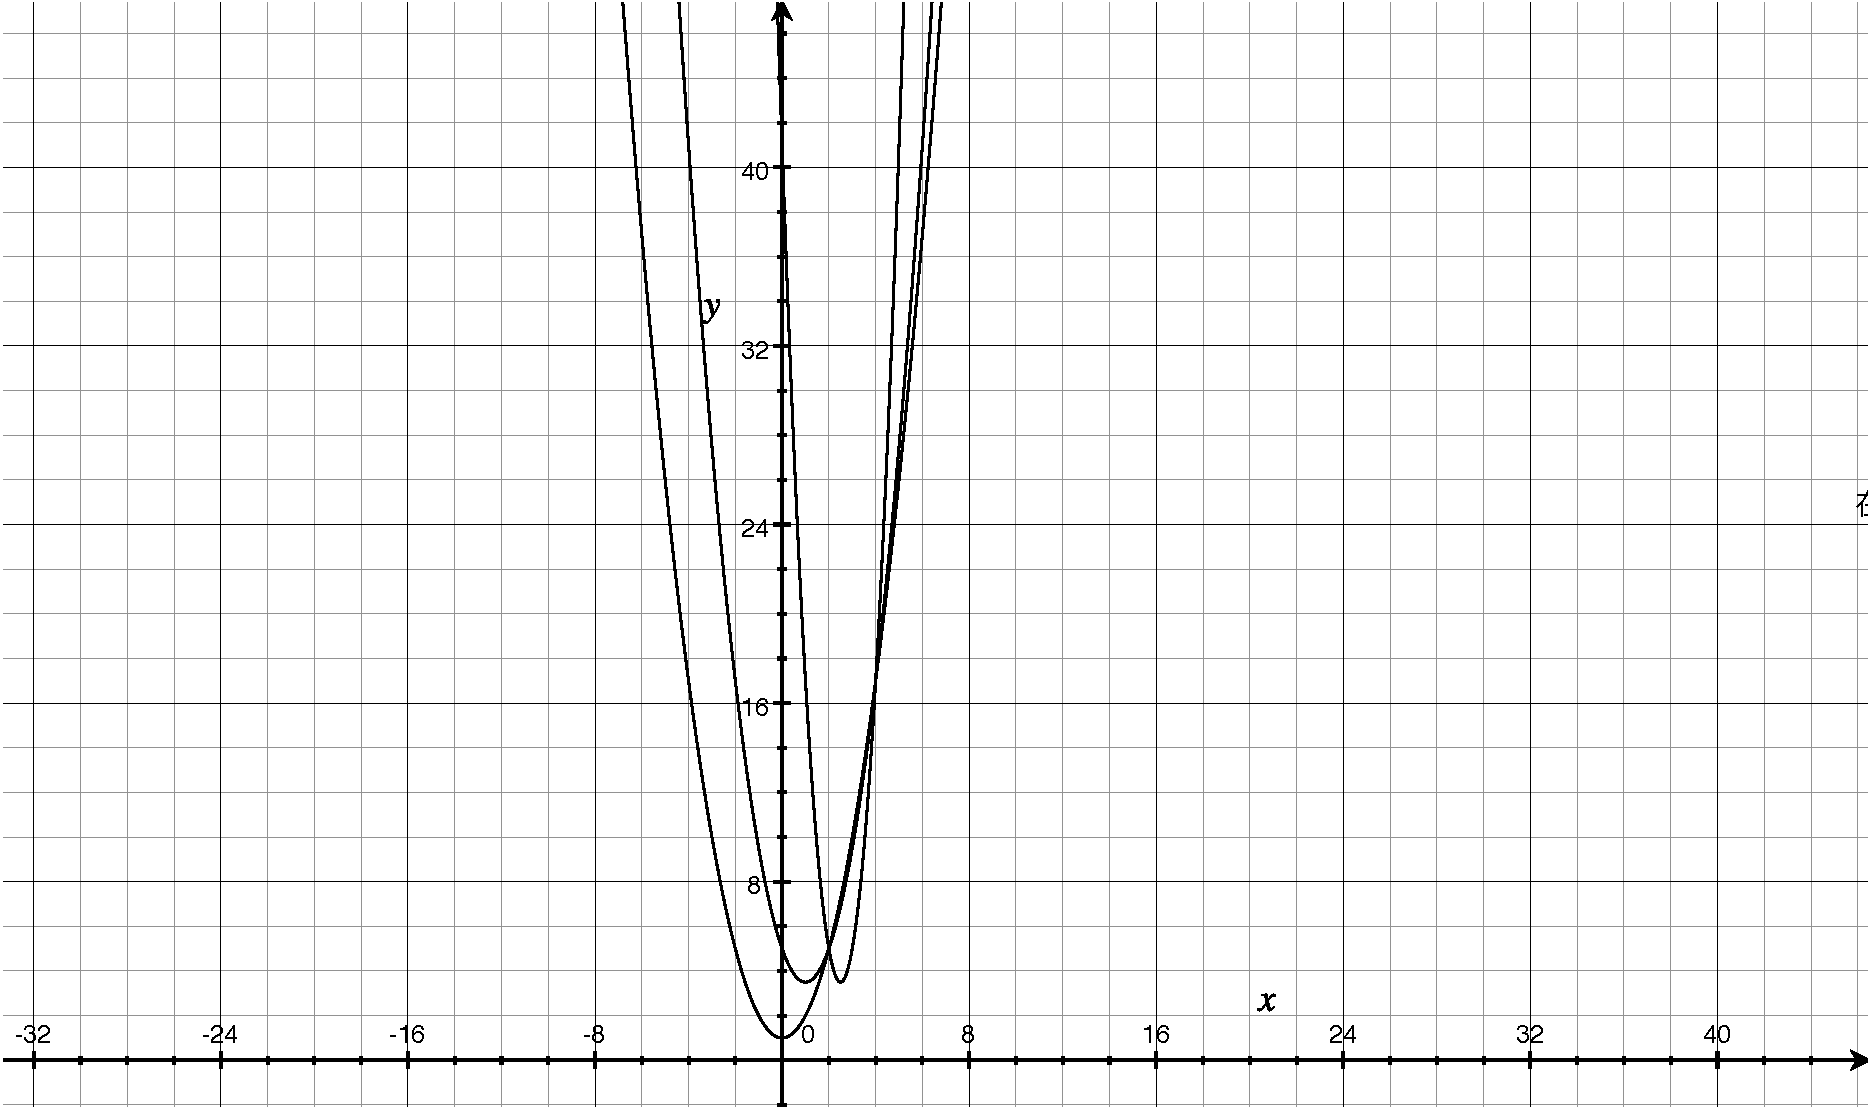
\includegraphics[width=0.75\textwidth]{images/5-1-b}
        \caption{\(L(x,\lambda) \, \text{versus x with positive}\, \lambda\)}
    \end{figure}

    \begin{figure}[h]
        \centering
            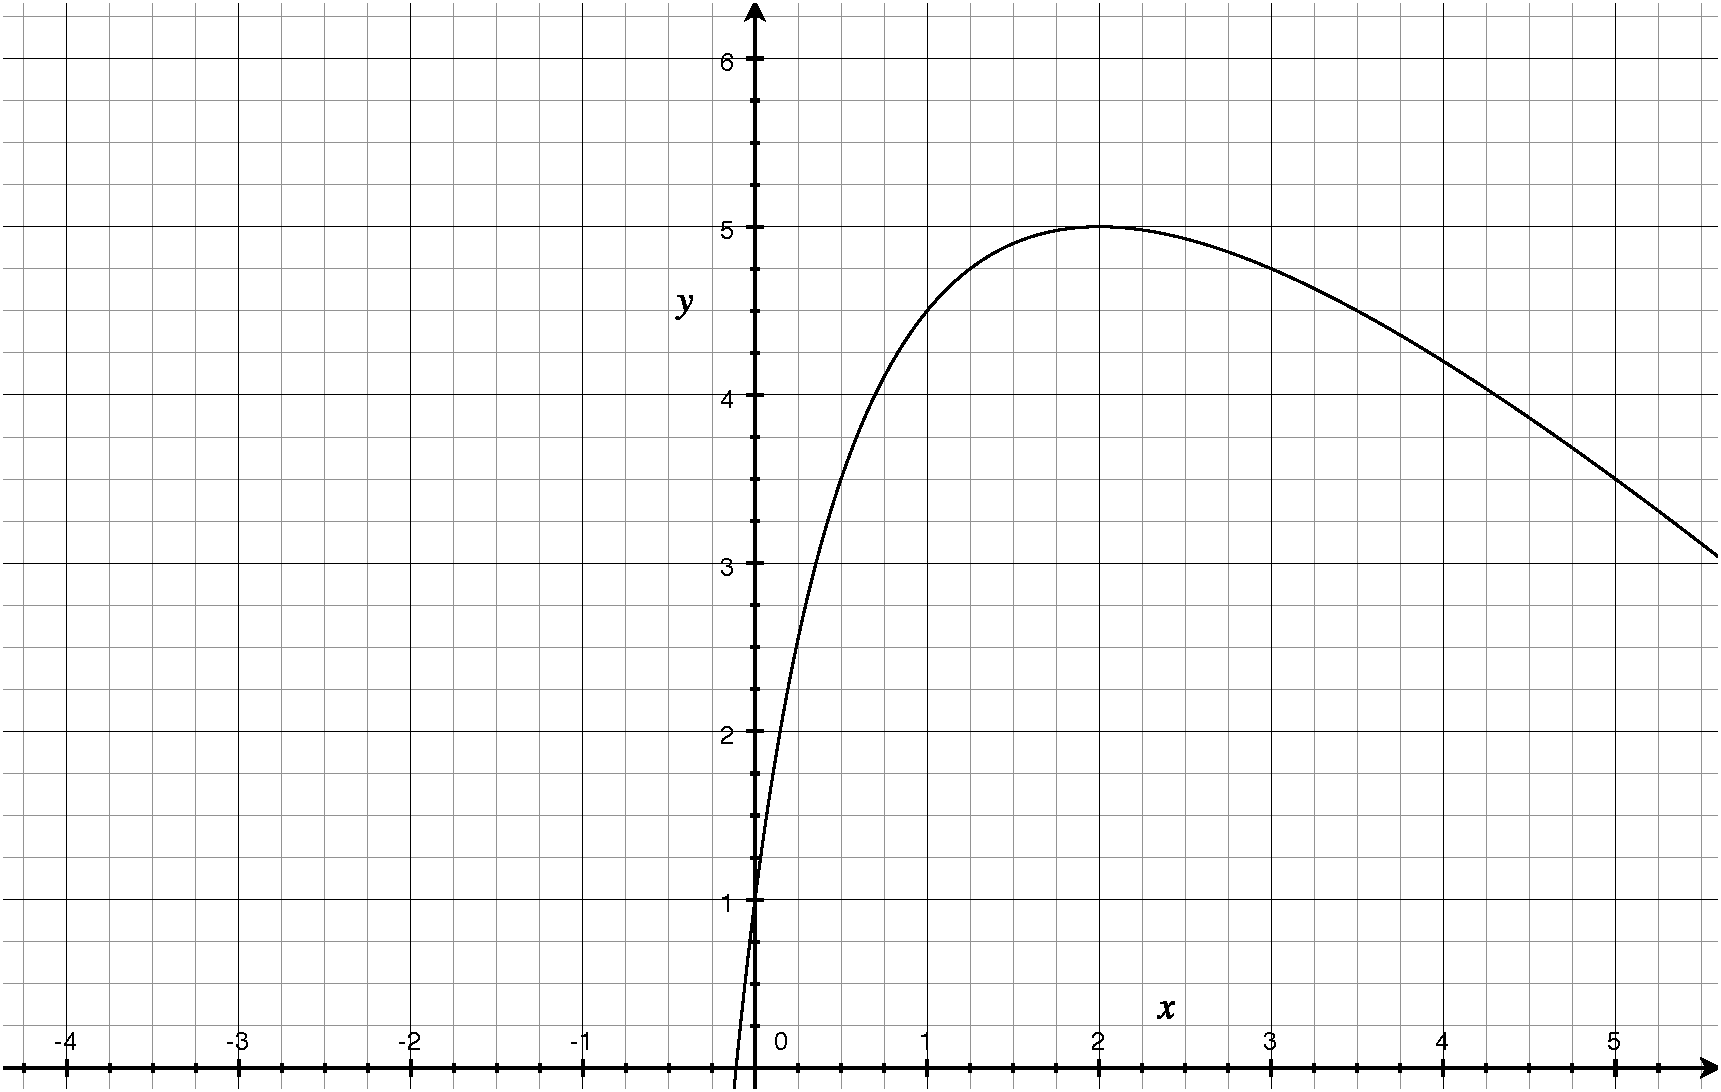
\includegraphics[width=0.75\textwidth]{images/5-1-b-2}
        \caption{\(g(\lambda) \; \text{versus} \; \lambda\)}
    \end{figure}

    (c) The Lagrange dual problem:
    \[ \begin{split}
        \text{maximize} \quad & \frac{9\lambda - \lambda^{2} + 1}{\lambda + 1} \\
        \text{subject to} \quad & \lambda \geq 0
        \end{split}
    \]
    It is a concave maximization problem and strong duality holds for it.
    And the optimal value:
    \[
        d^{\ast} = 5 \; \text{when} \; \lambda = 2
    \]

    (d) The feasible set is empty when \(u < -1\). When \(u \geq -1\), the feasible set is \([3-\sqrt{1+u}, 3 + \sqrt{1+u}] \). And the \(P^{\ast} = 11 + u - 6\sqrt{1+u} \) when \(-1 \leq u \leq 8\), \(P^{\ast} = 1\) when \(u > 8\). Thus
    \[
        p^{\ast} = \left\{\begin{array}{lc}
        \infty & u < -1 \\
        11 + u - 6\sqrt{1+u} & -1 \leq u \leq 8 \\
        1 & u > 8
        \end{array}\right.
    \]
    \begin{figure}[!h]
        \centering
            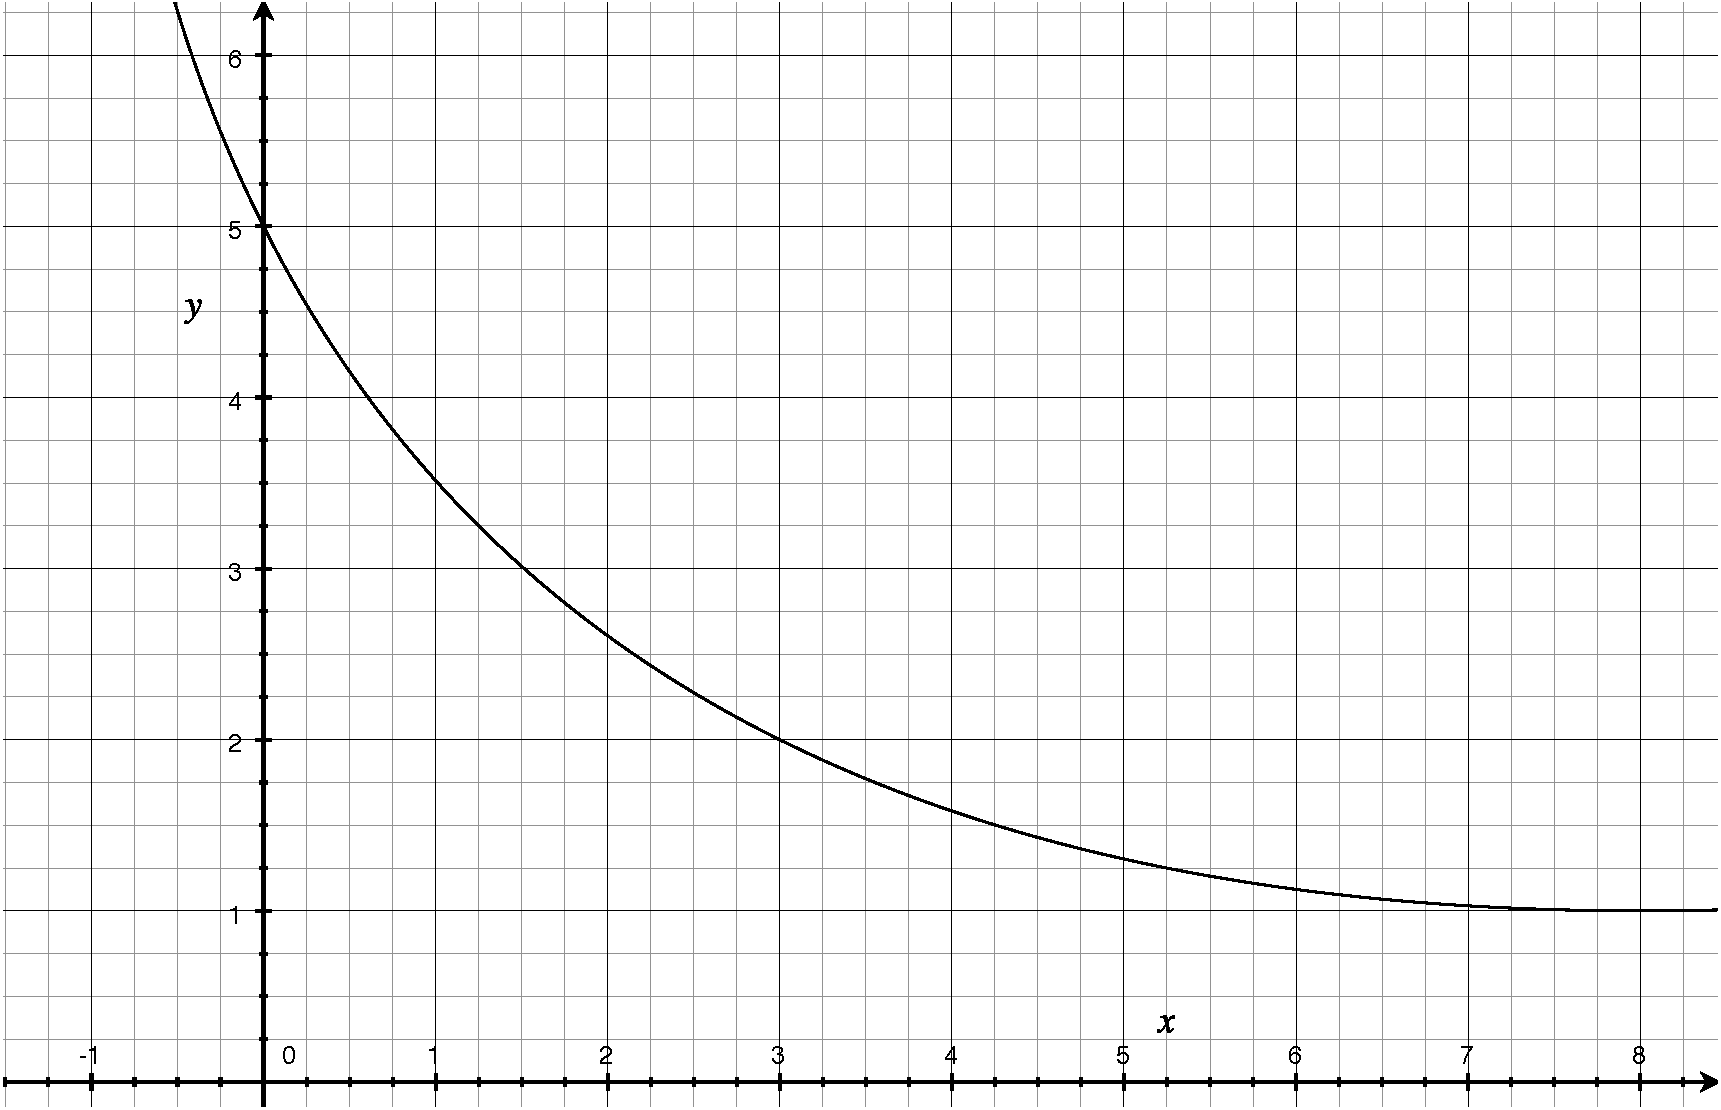
\includegraphics[width=0.75\textwidth]{images/5-1-d}
        \caption{\(p^{\ast}(u) \; \text{versus} \; u\)}
    \end{figure}


\end{homeworkProblem}

\pagebreak


\begin{homeworkProblem}
    Textbook exercise 5.13
    \\

    \solution

    (a) The Lagrange dual function is:
    \[
        \begin{split}
        g(\lambda, \nu) &= \inf_{x}\left(c^{T}x + \lambda^{T}(Ax - b) + \sum_{i} \nu_{i}(x_{i} - x_{i}^{2})\right) \\
        & = \inf_{x}\left(c^{T}x + \lambda^{T}(Ax - b) + \nu^{T}x - x^{T}diag(\nu)x\right) \\
        & = \inf_{x}\left(\sum_{i}^{n} ((c_{i} + a_{i}^{T}\lambda_{i} + \nu_{i})x_{i} + \nu_{i}x_{i}^{2}) - \lambda^{T}b\right) \\
        & = \left\{\begin{array}{lc} \sum_{i}^{n}\frac{-(c_{i}+a_{i}^{T}\lambda_{i}-\nu_{i})^{2}}{4\nu_{i}} - \lambda ^{T}b & \nu_{i} \geq 0 \\ -\infty & o.w.\end{array}\right.
        \end{split}
    \]
    And the dual problem is:
    \[
        \begin{split}
        \text{maximize}& \quad \sum_{i}^{n}\frac{-(c_{i}+a_{i}^{T}\lambda_{i}-\nu_{i})^{2}}{4\nu_{i}} - \lambda ^{T}b \\
        \text{subject to} &\quad \lambda \succeq 0, \; \nu \succeq 0
        \end{split}
    \]

    (b)The dual function of the LP relaxation is:
    \[
        \begin{split}
            g(x,\lambda_{1},\lambda_{2},\lambda_{3}) &= \inf_{x}(c^{T}x + \lambda_{1}^{T}(Ax-b) - \lambda_{2}^{T} x + \lambda_{3}^{T}(x- \mathbf{1})) \\
            & = \left\{\begin{array}{lc} -\lambda_{1}^{T}b + \lambda_{3}^{T} \mathbf{1} & c + A^{T}\lambda_{1} - \lambda_{2} + \lambda_{3} = 0 \\
            -\infty & o.w. \end{array} \right.
        \end{split}
    \]
    And the dual problem is:
    \[
        \begin{split}
            \text{maximize} \quad &-\lambda_{1}^{T}b + \lambda_{3}^{T} \mathbf{1} \\
            \text{subject to} \quad &c + A^{T}\lambda_{1} - \lambda_{2} + \lambda_{3} = 0 \\
            & \lambda_{1} \succeq 0, \; \lambda_{2} \succeq 0, \; \lambda_{3} \succeq 0
        \end{split}
    \]
    Thus, they can give the same lower bound.

\end{homeworkProblem}
\pagebreak

\begin{homeworkProblem}
    Textbook exercise 5.21
    \\

    \solution

    (a)It is a convex optimization problem. And the feasiable set is \(\{ (x,y)\;|\;x=0,\,y>0\}\). Thus the optimal value \(p^{\ast} = 1\).

    (b) The Lagrange dual function is:
    \[
        \begin{split}
        g(\lambda) &= \inf_{x \in \mathbf{D}}(e^{-x} + \lambda x^{2}/y) \\
        &= \left\{\begin{array}{lc} 0 & \lambda \geq 0 \\
        -\infty & \lambda < 0 \end{array}\right.
        \end{split}
    \]
    And the dual problem:
    \[
        \begin{split}
        \text{maximize} \quad & 0 \\
        \text{subject to} \quad & \lambda \geq 0
        \end{split}
    \]
    \(d^{\ast} = 0 \) and the duality gap \(p^{\ast} - d^{\ast} = 1\)

    (c)it is not satisfied.

    (d)
    \[
        p^{\ast} = \left\{ \begin{array}{lc} -\infty & u <0 \\
        1 & u=0\\
        0 & u> 0\end{array}\right.
    \]

   \( d^{\ast} \) is achieved when \( \lambda \geq 0 \). So the global sensitivity inequality does not hold apparently.
\end{homeworkProblem}
\pagebreak

\begin{homeworkProblem}
    Textbook exercise 5.27
    \\

    \solution

    (a)
    The KKT conditions for this problem is:

    \begin{equation}
    \label{eq:1}
        G^{T}x^{\ast} - h = 0
    \end{equation}
    \begin{equation}
        2A^{T}(Ax^{\ast} - b) + G^{T} \nu^{\ast}=0
    \end{equation}

    The Lagrangian is
    \begin{equation}
        \begin{split}
        L(x, \nu) &= \Vert Ax-b \Vert_{2}^{2} + \nu^{T}(Gx-h) \\
                  &= x^{T}A^{T}Ax + (G^{T}\nu - 2A^{T}b)^{T}x - 2\nu^{T}h
        \end{split}
    \end{equation}
    And the dual function is
    \begin{equation}
        g(\nu) = \inf_{x} ( L(x, \nu))
    \end{equation}
    which is a object function of a unconstrained least-squares problem. Let \(\nabla L(x, \nu) = 0\), we can get \(x_{1} = -\frac{1}{2}(A^{T}A)^{-1}(G^{T}\nu - 2A^{T}b)\). Thus, the dual function is equivalent to
    \begin{equation}
        g(\nu) = L( x_{1}, \nu)
    \end{equation}

    From equation \ref{eq:1}, we can get \(x^{\ast} = (A^{T}A)^{-1}(A^{T}b-\frac{1}{2}G^{T}\nu^{\ast})\), where \(\nu^{\ast} \;\text{satisfies}\; G^{T}(A^{T}A)^{-1}(A^{T}b-\frac{1}{2}G^{T}\nu^{\ast}) = h\)

\end{homeworkProblem}
\pagebreak
\begin{homeworkProblem}
    Textbook exercise 5.32
    \\

    \solution

    Let function \(g(x, u, \nu) = f_{0}(x)\) and \(\mathbf{dom} \;g = \{x,u,\nu \;|\; f_{i}(x) \leq u_{i},\; i=1,\dots,m, \; Ax-b= \nu\}\). Apparently the \(g(x, u, \nu)\) is convex on its domain. Therefore, the minimization of convex function \(p^{\ast}(u, \nu) = \inf_{x} g(x, u, \nu)\) is convex on its domain.


\end{homeworkProblem}
\pagebreak

\begin{homeworkProblem}
    Textbook exercise 5.39
    \\

    \solution

    (a)
    If \(X\) is feasible, \(X\) can be expressed as \(xx^{T}\) because of \( \mathbf{rank}\; X = 1\). \(X_{ii} =1 \) is equivalent to \(x_{i} \in \{-1,1\}\) because \((xx^{T})_{ij} = x_{i}x_{j}\).
    \(\mathbf{tr}\{WX\} = x^{T}Wx\).

    If \(x_{i}^{2} = 1, i=1,\dots,n\), let \(X = xx^{T}\) and we can get \(X_{ii} = x_{i}^{2}, \; \mathbf{rank} \; X =1\).

    (b)Its optimal value gives a lower bound because we minimize the object function on a relaxed constrains. It's primal optimal when the \(\mathbf{rank} \;X^{\ast} = 1\).

    (c)The SDP relaxation is equivalent to
    \[
        \begin{split}
        \text{minimize} &\quad 1^{T}\nu \\
        \text{subject to} & \quad W + \mathbf{diag}(\nu) \geq 0
        \end{split}
    \]
    Its dual function is
    \[
        \begin{split}
        g(\nu, X) &= \inf_{x}(1^{T} - \mathbf{tr}(X(W + \mathbf{diag}(\nu))) \\
        &= \inf_{x}(-\mathbf{tr}(XW) + \sum_{i=1}^{n}\nu_{i}(1-X_{ii})) \\
        &=
        \left\{
        \begin{array}{lc} -\mathbf{tr}(XW) & X_{ii} =1, i=1,\dots,n \\ -\infty & o.w.\end{array}
        \right.
        \end{split}
    \]
    Thus, its dual problem is
    \[
        \begin{split}
        \text{maximize} &\quad -\mathbf{tr}(XW) \\
        \text{subject to} &\quad X \succeq 0 \\
        & \quad X_{ii} = 1, \;i=1,\dots,n
        \end{split}
    \]
    which is equivalent to the (5.114). The lower bounds found by it is better than those found by (5.114).

\end{homeworkProblem}


\end{document}
